\documentclass[12pt]{exam}
\usepackage[utf8]{inputenc}

\usepackage{amsmath,amstext,amsthm,amssymb,amsxtra}
\usepackage[top=1.5in, bottom=1.5in, left=1.25in, right=1.25in]	{geometry}
%\usepackage[normalem]{ulem}
\usepackage{txfonts} % pxfonts txfonts 
\usepackage[T1]{fontenc}
\usepackage{lmodern}
\renewcommand*\familydefault{\sfdefault}
 \usepackage{euler}   % better than the option below
\usepackage{pdfsync}
\usepackage{multicol}
\newcommand{\ci}[1]{_{ {}_{\scriptstyle #1}}}
\usepackage{graphicx}
\graphicspath{ {images/} }


\newcommand{\norm}[1]{\ensuremath{\left\|#1\right\|}}
\newcommand{\abs}[1]{\ensuremath{\left\vert#1\right\vert}}
\newcommand{\ip}[2]{\ensuremath{\left\langle#1,#2\right\rangle}}
\newcommand{\p}{\ensuremath{\partial}}
\newcommand{\pr}{\mathcal{P}}

\newcommand{\pbar}{\ensuremath{\bar{\partial}}}
\newcommand{\db}{\overline\partial}
\newcommand{\D}{\mathbb{D}}
\newcommand{\B}{\mathbb{B}}
\newcommand{\Sp}{\mathbb{S}}
\newcommand{\T}{\mathbb{T}}
\newcommand{\R}{\mathbb{R}}
\newcommand{\Z}{\mathbb{Z}}
\newcommand{\C}{\mathbb{C}}
\newcommand{\N}{\mathbb{N}}
\newcommand{\Q}{\mathbb{Q}}
\newcommand{\mQ}{\mathcal{Q}}
\newcommand{\mS}{\mathcal{S}}
\newcommand{\scrH}{\mathcal{H}}
\newcommand{\scrL}{\mathcal{L}}
\newcommand{\td}{\widetilde\Delta}
\newcommand{\pw}{\text{PW}}
\newcommand{\esup}{\text{ess.sup}}
\newcommand{\Tn}{\mathcal{T}_n}
\newcommand{\Bn}{\mathbb{B}_n}
\newcommand{\rt}{\mathcal{O}}
\newcommand{\avg}[1]{\langle #1 \rangle}
\newcommand{\one}{\mathbbm{1}}
\newcommand{\eps}{\varepsilon}
\newcommand{\grad}{\nabla}

\newcommand{\La}{\langle }
\newcommand{\Ra}{\rangle }
\newcommand{\rk}{\operatorname{rk}}
\newcommand{\card}{\operatorname{card}}
\newcommand{\ran}{\operatorname{Ran}}
\newcommand{\osc}{\operatorname{OSC}}
\newcommand{\im}{\operatorname{Im}}
\newcommand{\re}{\operatorname{Re}}
\newcommand{\tr}{\operatorname{tr}}
\newcommand{\vf}{\varphi}
\newcommand{\f}[2]{\ensuremath{\frac{#1}{#2}}}

\newcommand{\kzp}{k_z^{(p,\alpha)}}
\newcommand{\klp}{k_{\lambda_i}^{(p,\alpha)}}
\newcommand{\TTp}{\mathcal{T}_p}
\newcommand{\m}[1]{\mathcal{#1}}
\newcommand{\md}{\mathcal{D}}
\newcommand{\qan}{\abs{Q}^{\alpha/n}}
\newcommand{\sbump}[2]{[[ #1,#2 ]]}
\newcommand{\mbump}[2]{\lceil #1,#2 \rceil}
\newcommand{\cbump}[2]{\lfloor #1,#2 \rfloor}

\newcommand{\class}{Math 629 Spring 26}
\newcommand{\term}{Fall 24}
\newcommand{\examnum}{Homework \hwnum}
\newcommand{\examdate}{\duedate}
\newcommand{\timelimit}{75 Minutes}
\newcommand{\vc}[3]{\langle #1,#2,#3\rangle}
\newcommand*{\vv}[1]{\vec{\mkern0mu#1}}
\newcommand{\bv}[1]{\boldsymbol{#1}}
\newcommand{\hide}[1]{}
\newcommand{\uvec}[1]{\boldsymbol{\hat{\textbf{#1}}}}
\newcommand{\vex}[1]{\boldsymbol{{\textbf{#1}}}}

\pagestyle{head}
\firstpageheader{}{}{}
\runningheader{\class}{\examnum\ - Page \thepage\ of \numpages}{\examdate}
\runningheadrule

\makeatletter
\renewcommand*\env@matrix[1][*\c@MaxMatrixCols c]{%
  \hskip -\arraycolsep
  \let\@ifnextchar\new@ifnextchar
  \array{#1}}
\makeatother

%\printanswers
\begin{document}

\noindent
\begin{tabular*}{\textwidth}{l @{\extracolsep{\fill}} r @{\extracolsep{6pt}} l}
\textbf{\class} & \textbf{Name: Mengxiang Jiang}\\
\end{tabular*}\\
\rule[2ex]{\textwidth}{2pt}
%

 

\newcommand{\duedate}{02/09/2026 at 11:59pm}
\newcommand\hwnum{3}

Turn this assignment in on gradescope. All work must be neat and legible. Turn in 
a ``final draft''. There should be nothing scratched out and your work should flow
generally from left to right and top to bottom. 

\begin{questions}
\question
Using the chord function, find the side length of a 12-gon inscribed in a circle
of radius $1$. Find a general formula for the side length of a $2^k 6$-gon inscribed
in a circle of radius $1$. 
\\\\
Since a 12-gon has 12 angles, the central angle $\alpha$ subtended by each side is 
$\frac{360^\circ}{12} = 30^\circ$.
Therefore the side length $s$ of the 12-gon is just crd($30^\circ$).
\\\\
For a $2^k 6$-gon, the central angle $\alpha$ subtended by each side is 
$\frac{360^\circ}{2^k 6} = \frac{60^\circ}{2^k}$.
Therefore the side length $s$ of the $2^k 6$-gon is just crd($\frac{60^\circ}{2^k}$).


\newpage
\question 
Consider three points $A,B,C$ on a circle with center $O$. For simplicity, take 
$A,B$ to be in the first quadrant with $A$ lower than $B$ and $C$ in the third quadrant.
What is the relation between $\angle AOB$ and $\angle ACB$?
\\\\
Since $A$, $B$, and $C$ are on the same circle, the angle $\angle ACB$ is 
an inscribed angle that subtends the same arc as the central angle $\angle AOB$.
By the inscribed angle theorem, we have $\angle ACB = \frac{1}{2} \angle AOB$.

\newpage 
\question 
Given a square, hexagon, and circle with the same perimeter, which one encloses the
most area? Which one encloses the least? Provide an argument for this using methods
we've seen in class (by this, really I just want you to think ``geometrically'' 
or even ``trigonometrically'' and not use more advanced theorems from -- say -- 
calculus). 
\\\\
Let the common perimeter be $P$. I'll use the results from the previous homework where
the area of a regular $n$-gon is $A = \frac{1}{2}Pa$, where $a$ is the apothem of 
the regular $n$-gon. Now we just need to relate the apothem to the 
number of sides $n$ and the perimeter $P$.
\\\\
First note that we can always divide a regular $n$-gon into $n$ 
congruent isosceles triangles by drawing segments from the center to the vertices. 
Each of these triangles has a base of length $\frac{P}{n}$ and 
an apex angle (in radians) of $\frac{2\pi}{n}$. If we bisect the apex angle, 
we get two right triangles with an angle of $\frac{\pi}{n}$. 
Then we can express the apothem $a$ in terms of the base and this angle:
\begin{align*}
  \tan\left(\frac{\pi}{n}\right) &= \frac{\frac{P}{2n}}{a}\\
  a &= \frac{P}{2n\tan\left(\frac{\pi}{n}\right)}\\
  a &= \frac{P}{2n}\cot\left(\frac{\pi}{n}\right)
\end{align*}
Therefore the area of a regular $n$-gon with perimeter $P$ is
\begin{align*}
  A &= \frac{1}{2}Pa\\
  &= \frac{1}{2}P \cdot \frac{P}{2n}\cot\left(\frac{\pi}{n}\right)\\
  &= \frac{P^2}{4n}\cot\left(\frac{\pi}{n}\right)
\end{align*}
Without going into calculus, we will compare the rates of growth of the 
area as $n$ increases by looking at the behavior of 
$\frac{\cot\left(\frac{\pi}{n}\right)}{n}$ as $n$ increases, 
since $\frac{P^2}{4}$ is the same for every $n$-gon.
One key fact to note is that 
\[
  x < \tan x \quad \text{for } 0 < x < \frac{\pi}{2}.
\]
We show this through a visual geometric argument. Consider the unit circle 
and the tangent line to the circle at the point $A:(1,0)$.
\begin{center}
    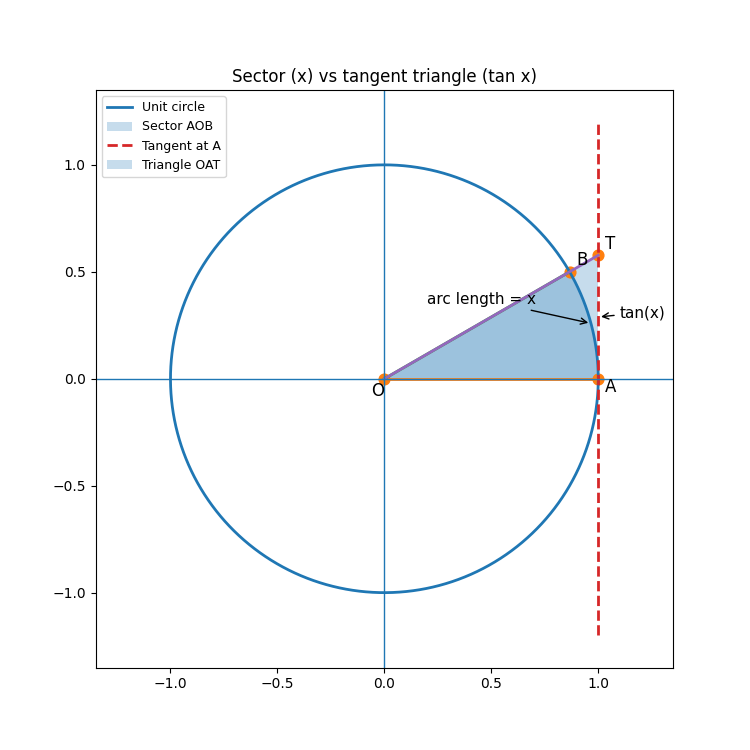
\includegraphics[width=0.8\textwidth]{tanx.png}
\end{center}
The length of the arc from $A$ to the point on the unit circle corresponding 
to an angle $x$ is exactly $x$ (by the definition of radian measure).
The length of the segment from $A$ to the point on the tangent line corresponding
to the same angle $x$ is exactly $\tan x$. The area of the sector
is $\frac{x}{2\pi} \cdot \pi = \frac{x}{2}$, 
and the area of the triangle formed by the tangent line 
and the two radii is $\frac{\tan x}{2}$. 
Since the sector is contained within the triangle, 
we have $\frac{x}{2} < \frac{\tan x}{2}$ for $0 < x < \frac{\pi}{2}$.
Now we can use this fact to compare the growth rates 
of $\frac{\cot\left(\frac{\pi}{n}\right)}{n}$ as $n$ increases. 
We have
\begin{align*}
  \frac{\cot\left(\frac{\pi}{n}\right)}{n} &= 
  \frac{1}{n\tan\left(\frac{\pi}{n}\right)}\\
  &< \frac{1}{n \cdot \frac{\pi}{n}}\\
  &= \frac{1}{\pi}
\end{align*}
As $n$ increases, $\frac{\cot\left(\frac{\pi}{n}\right)}{n}$ 
approaches $\frac{1}{\pi}$ from below, 
which means that the area of the regular $n$-gon approaches $\frac{P^2}{4\pi}$ 
from below as $n$ increases. If we substitute $P=2\pi r$ for the circle, 
we get the expected area of the circle of $\pi r^2$, which is the 
upper bound of the area of the regular $n$-gon as $n$ increases.
Therefore, among the square, hexagon, and circle with the same perimeter, 
the circle encloses the most area, while the square encloses the least area.

\newpage 
\question 
Find the volume of a torus by applying Pappus's Theorem. Assume that the torus is formed
by revolving the disk of radius $r$ around an axis whose distance from the center
of the disk is $R > r$.
\\\\
Pappus's Theorem states that the volume of a solid of revolution generated 
by revolving a plane figure around an external axis is equal to the product 
of the area of the figure and the distance traveled by its centroid.
In this case, the plane figure is a disk of radius $r$, 
which has an area of $\pi r^2$. The centroid of the disk is at its center, 
which is a distance of $R$ from the axis of revolution. 
When the disk is revolved around the axis, the centroid travels a circular path 
with a circumference of $2\pi R$.
Therefore, the volume of the torus is given by:
\[
  V = \text{Area of disk} \times \text{Distance traveled by centroid} = \pi r^2 \times 2\pi R = 2\pi^2 R r^2.
\]

\end{questions}
\end{document}
